\section{Background and Methodology}
\label{sec:background}

We first trace the physical path of host-to-device posted MMIO writes across modern x86 server uncore and SmartNIC/accelerator silicon, then describe our dual-target testbed and hardware-counter methodology.

\begin{figure*}[t]
  \centering
  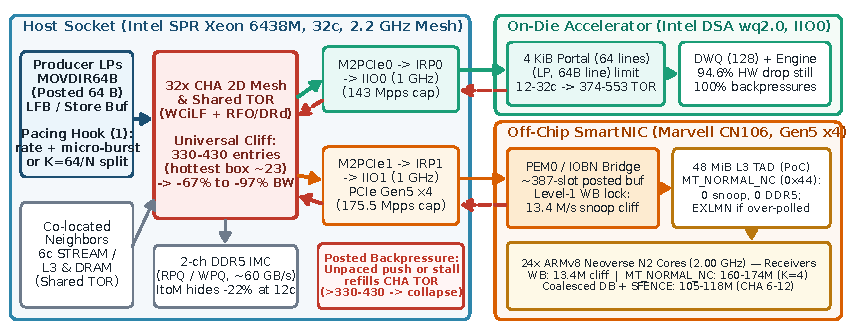
\includegraphics[width=\textwidth]{figures/fig0_architecture.pdf}
  \caption{End-to-end architecture of MMIO direct push across our dual-target Intel Sapphire Rapids testbed. Posted \texttt{MOVDIR64B} writes bypass the host LLC and DDR5 channels but allocate entries in the shared 32-slice \texttt{CHA TOR}. Unpaced host multi-core injection (on either \texttt{IIO0} Intel DSA or \texttt{IIO1} CN106 \texttt{BAR4}) or receiver-side stalls on CN106 (\texttt{Normal-WB} snoop locks or \texttt{MT\_NORMAL\_NC} \texttt{EXLMN} collisions) propagate posted backpressure upstream into \texttt{CHA TOR}, triggering socket-wide neighbor collapse once \texttt{WCiLF} exceeds 330--430 entries.}
  \label{fig:arch}
\end{figure*}

\subsection{Host-to-Device MMIO Push Microarchitecture}
\label{sec:bg_host}

On Intel Sapphire Rapids (SPR), each socket connects 32 Golden Cove cores, 32 Caching and Home Agent (\texttt{CHA}) slices, Integrated Memory Controllers (\texttt{IMC}), and Integrated I/O stacks (\texttt{IIO}) over a 2D mesh running at the uncore clock (2.20\,GHz locked in our experiments). Each \texttt{CHA} slice hosts a slice of the 60\,MiB non-inclusive LLC and a fixed-size Table of Requests (\texttt{TOR}) that tracks every active coherent memory transaction (\eg{} \texttt{DRd}, \texttt{RFO}, \texttt{ItoM}) \emph{and} every non-coherent MMIO transaction (\texttt{PRd}, \texttt{UCRdF}, \texttt{WCiLF}) mapped to that slice.

\para{Posted 64\,B writes (\texttt{MOVDIR64B}) vs. cacheable stores.}
Standard PCIe MMIO BARs cannot be mapped write-back (\texttt{WB}) on x86 Linux servers because three independent hardware and OS layers block it: Linux PAT sanitizes BAR mappings to \texttt{UC}/\texttt{WC}, MTRRs mark the PCIe MMIO hole uncachable, and the SPR System Address Decoder (\texttt{SAD}) routes MMIO addresses directly to \texttt{M2PCIe} without coherent directory ownership. Even if a write-combining (\texttt{WC}) BAR is flushed via \texttt{CLWB}, cache-line write-back instructions are weakly ordered relative to subsequent stores without an explicit \texttt{SFENCE}~\cite{intelmovdir2024}.

Instead, high-rate MMIO direct push uses \texttt{MOVDIR64B}~\cite{intelmovdir2024}: an atomic, 64-byte direct store that bypasses the core's L1/L2 caches and host LLC and emits a single 64-byte posted Write-Combining Invalidate Line Full (\texttt{WCiLF}) transaction into the 2D mesh. Each \texttt{WCiLF} allocates a \texttt{TOR} entry in the home \texttt{CHA} slice determined by the destination physical address hash, traverses the mesh to the target stack's \texttt{M2PCIe} bridge (non-coherent bypass queue, \texttt{NCB}), enters the I/O Request Pipeline (\texttt{IRP}) and \texttt{IIO} root complex (1.00\,GHz clock domain), and exits as a posted PCIe Memory Write (\texttt{MWr}) TLP with Relaxed Ordering cleared (\texttt{RO\,=\,0} per x86 MMIO ordering rules~\cite{pcisig2019pcie5})---or enters an on-die accelerator portal such as Intel DSA~\cite{inteldsa2023}.

\para{Non-posted MMIO latency anatomy.}
To establish concrete hardware baselines on our SPR--CN106 link, we decomposed an isolated (\texttt{W\,=\,1}) 8\,B non-posted MMIO Read into six clock-domain-verified stages using non-multiplexed \texttt{CHA}, \texttt{M2PCIe1}, \texttt{IRP1}, \texttt{IIO1}, and CN106 \texttt{TAD}/\texttt{DDR5} counters combined with independent core/uncore frequency sweeps and Root Port (\texttt{98:01.0}) differential reads. Subtracting the 12.7\,ns \texttt{LFENCE;RDTSC} bracket floor, an isolated \texttt{BAR4} read hitting CN106's 48\,MiB L3 takes 621.8\,ns median (634.5\,ns for a single 64\,B \texttt{vmovdqu64} TLP; 715.5\,ns on L3 miss to card DDR5, a +93.6\,ns penalty with exactly 2.00 64\,B DDR5 bursts per 128\,B L3 line). Across the full path, host core front-end/LFB accounts for 10.5\,ns, core--CHA mesh outside \texttt{TOR} takes 10.8--12.9\,ns, \texttt{CHA TOR}\,$\leftrightarrow$\,\texttt{M2PCIe1} takes 58.6\,ns, \texttt{IRP1 + IIO1} takes 125.8\,ns, the PCIe Gen5\,$\times$4 link plus CN106 \texttt{PEM0}\,$\to$\,\texttt{SDP} adds +290.9\,ns warm (+312.1\,ns cold), and CN106 \texttt{BAR4\_INDEX + IOBN + TAD L3} adds +99.2--105.2\,ns. Posted \texttt{MOVDIR64B} writes avoid the completion half of this round trip, achieving an unloaded host--card--host echo RTT of 889--902\,ns when paired with write-combining outbound replies.

\subsection{Dual Silicon Targets and Device Memory Semantics}
\label{sec:bg_targets}

A recurring concern in hardware-characterization studies is whether observed bottlenecks are quirks of a single peripheral. We therefore evaluate posted MMIO direct push across two architecturally distinct targets attached to \emph{separate \texttt{IIO} stacks} of the same Sapphire Rapids socket (\autoref{tab:platform}):

\begin{table}[t]
  \centering
  \scriptsize
  \setlength{\tabcolsep}{3.5pt}
  \begin{tabularx}{\columnwidth}{@{}l Y@{}}
    \toprule
    \textbf{Component} & \textbf{Configuration \& Fixed Experimental Baseline} \\
    \midrule
    Host CPU & Dual-socket Intel Xeon Gold 6438M (SPR); all active tests isolated to Socket~1 (32 physical cores \texttt{cpu32..63}, 32 SMT \texttt{cpu96..127}), 60\,MiB LLC, uncore locked at 2.20\,GHz, \texttt{cpu40} at 3.90\,GHz (\texttt{performance}), 2-ch DDR5 (\(\sim\)60\,GB/s). \\
    Target 1 (Off-chip) & Marvell OCTEON~10 CN106 SmartNIC on Socket~1 \texttt{IIO1} (PCIe Gen5\,$\times$4, 32\,GT/s, 175.5\,Mpps posted ceiling): 24 ARMv8 Neoverse N2 cores (2.00\,GHz), 64\,KiB L1D / 1\,MiB L2 per core, 48\,MiB shared L3 (\texttt{TAD}, 128\,B lines, CHI PoC), 6-ch DDR5, 4\,MiB \texttt{BAR4} slot~15 (32,768 $\times$ 64\,B lines). \\
    Target 2 (On-die) & Intel DSA \texttt{dsa2/wq2.0} (\texttt{0000:f2:01.0}) on Socket~1 \texttt{IIO0}: dedicated work queue (128 entries, 1 or 4 engines), 4\,KiB portal (64 $\times$ 64\,B lines), 143\,Mpps posted ceiling. \\
    Peer Host (100\,GbE) & Dedicated load generator (\texttt{mercury}) connected over 100\,GbE (NVIDIA ConnectX-6 / \texttt{mlx5} $\leftrightarrow$ CN106 100\,GbE \texttt{eth0}) for end-to-end KV and Memcached evaluation. \\
    PMU Audit & 100\% non-multiplexed hardware counters (\texttt{min\_pct\,=\,100\%}): SPR \texttt{32$\times$CHA TOR} (\texttt{all}/\texttt{WCiLF}), \texttt{M2PCIe0/1}, \texttt{IRP0/1}, \texttt{IIO0/1}, \texttt{IMC RPQ/CAS}; CN106 \texttt{armv8\_pmuv3} (\texttt{l1d\_refill}, \texttt{0x58 L2D\_CACHE\_INVAL}), \texttt{TAD}, \texttt{DDR5}. Zero page faults, zero EDAC/AER increments. \\
    \bottomrule
  \end{tabularx}
  \caption{Dual-target hardware platform and non-multiplexed PMU auditing baseline.}
  \label{tab:platform}
\end{table}

\para{Target 1: Off-chip CN106 SmartNIC (\texttt{IIO1}, \texttt{BAR4}).}
CN106 exposes a 4\,MiB window (\texttt{BAR4} slot~15, 32,768 distinct 64\,B lines) mapped directly into card memory via PCIe Gen5\,$\times$4. Inbound PCIe posted writes enter the card's PCIe Endpoint Module (\texttt{PEM0}) and I/O Bridge (\texttt{IOBN}), which enforces PCIe posted ordering and injects coherent writes into CN106's 48\,MiB shared L3 (\texttt{TAD}, the ARM CHI Point of Coherence). By default, Linux maps card-side ring buffers as cacheable Write-Back (\texttt{Normal-WB}, \texttt{MAIR\_EL1} attribute \texttt{0xFF}), pulling polled slots into each ARM core's private 64\,KiB L1D and 1\,MiB L2. We also evaluate remapping the ring with standard Linux \texttt{MT\_NORMAL\_NC} (\texttt{0x44}) without modifying \texttt{MAIR\_EL1}, verified via ARMv8 \texttt{AT S1E0R}/\texttt{PAR\_EL1} hardware address translation.

\para{Target 2: On-die Intel DSA Portal (\texttt{IIO0}, 4\,KiB).}
Intel DSA exposes a single 4\,KiB (64-line) dedicated work queue (\texttt{DWQ}) portal on Socket~1 \texttt{IIO0}~\cite{inteldsa2023}. Host cores submit 64\,B descriptors using \texttt{MOVDIR64B}. Unlike a PCIe endpoint that backpressures indefinitely when full, a DSA \texttt{DWQ} discards overflow descriptors in hardware and logs \texttt{SWERROR}. Testing DSA alongside CN106 lets us cleanly separate off-chip PCIe link effects from on-die \texttt{IIO}/\texttt{CHA} mechanics, and test whether hardware descriptor dropping or narrow 4\,KiB portal windows immunize the host against \texttt{CHA TOR} contention.

\para{Measurement discipline.}
All microbenchmarks lock Socket~1 uncore frequency to 2.20\,GHz, pin coordinator threads to Socket~0 (\texttt{cpu0}), bind memory with \texttt{MPOL\_BIND} and pre-faulted hugepages (0 page faults), interleave $n\,=\,3$ repetitions per configuration, and enforce 100.0\% non-multiplexed PMU scheduling on both host and SmartNIC. Every multi-core interference test includes a core-count-matched \texttt{l1-spin} control that reproduces the exact multi-core turbo frequency drop (3.90\,$\to$\,3.25\,$\to$\,2.80\,GHz) so frequency scaling is never conflated with interconnect contention.
